\documentclass[]{article}
\usepackage {amsmath}
\usepackage[a4paper, total={7.3in, 10.3in}]{geometry}
\usepackage{cleveref}

\usepackage[titletoc]{appendix}
\usepackage{lmodern}

\makeatletter
\ifcase \@ptsize \relax% 10pt
  \newcommand{\miniscule}{\@setfontsize\miniscule{4}{5}}% \tiny: 5/6
\or% 11pt
  \newcommand{\miniscule}{\@setfontsize\miniscule{5}{6}}% \tiny: 6/7
\or% 12pt
  \newcommand{\miniscule}{\@setfontsize\miniscule{5}{6}}% \tiny: 6/7
\fi
\makeatother

\usepackage{lipsum}
\usepackage{amssymb}
%\usepackage{xcolor}
\usepackage[x11names, rgb]{xcolor}
\usepackage[utf8]{inputenc}
\usepackage{mathtools}
\usepackage{xcolor}
\usepackage{braket}
\usepackage{ulem}
\usepackage{cancel}
\usepackage{graphicx}
\usepackage{mathtools}
\usepackage{amsmath}  
\usepackage{amsfonts} 
\usepackage{graphicx}
\usepackage{amssymb} 
\usepackage{amsmath}
\usepackage{mathrsfs}
\usepackage{empheq}
\usepackage{amsthm}
 \usepackage{braket}
 \usepackage{amsmath}
\DeclareMathOperator\arctanh{arctanh}
\usepackage[utf8]{inputenc}
\usepackage[english]{babel}
\usepackage{graphicx}
\newtheorem{theorem}{Theorem}[section]
\newtheorem{corollary}{Corollary}[theorem]
\newtheorem{lemma}[theorem]{Lemma}
\numberwithin{equation}{section}
\newcommand{\pd}[2]{\frac{\partial{#1}}{\partial{#2}}}
\newcommand{\Cc}{\mathbb{C}}
\newcommand{\Ss}{\mathbb{S}}
% \newcommand{\Qq}{\mathrm{q}}
\newcommand{\pT}{\hat{+}}
\newcommand{\mT}{\hat{-}}
\newcommand{\muT}{\hat{\mu}}
\newcommand{\nuT}{\hat{\nu}}
\newcommand{\alphaT}{\hat{\alpha}}
\newcommand{\betaT}{\hat{\beta}}
\newcommand{\sigmaT}{\hat{\sigma}}
\newcommand{\rhoT}{\hat{\rho}}
\newcommand{\muL}{\tilde{\mu}}
\newcommand{\nuL}{\tilde{\nu}}
\newcommand{\uniT}[1]{\mathring{#1}}
\newcommand{\itP}[1]{\hat{#1}}
\newcommand{\lF}[1]{\tilde{#1}}
\newcommand{\Pp}{\mathbb{P}}
\newcommand{\Qq}{\mathbb{Q}}
\def\epp{\epsilon^{\prime}}
\def\ep{\epsilon}
\def\vep{\varepsilon}
\def\la{\langle}
\def\ra{\rangle}
\def\ppg{\pi^+\pi^-\gamma}
\def\vp{{\bf p}}
\def\ko{K^0}
\def\kb{\bar{K^0}}
\def\ka{\kappa}
\def\al{\alpha}
\def\ab{\bar{\alpha}}
\def\be{\begin{equation}}
\def\ee{\end{equation}}
\def\bea{\begin{eqnarray}}
\def\eea{\end{eqnarray}}
\def\wh{\widehat}


\title{$\mathbb{Z}_2$ lattice gauge theory}
\author{\textbf{Hariprashad Ravikumar}} 

\date{(For Dr. Engelhardt's meeting on July 14, 2022)}
\begin{document}
	\maketitle


\section{Gauge theory as a theory of phases}
Consider the general gauge group $G$.
\begin{align}
    U_{ij}\in G
\end{align}
where $U_{ij}$ is an $n\times n$ matrix. 
\begin{align}
    U_{ij}&=P.O.\left(\exp{\left(ig_0\int_{x_i}^{x_j}A_{\mu}.dx_{\mu}\right)}\right)
\end{align}
The action should be a
sum over all elementary squares of the lattice,
\begin{align}
    S=\sum_\Box S_\Box
\end{align}
The action on each of these squares or 'plaquettes' is the trace of the product of the group elements surrounding the plaquette
\begin{align}
    S_\Box=\beta\left[1-\left(\frac{1}{n}\right)Re~Tr\left(U_{ij}U_{jk}U_{kl}U_{li}\right)\right]
\end{align}
\begin{figure}  [h!]
	\centering
	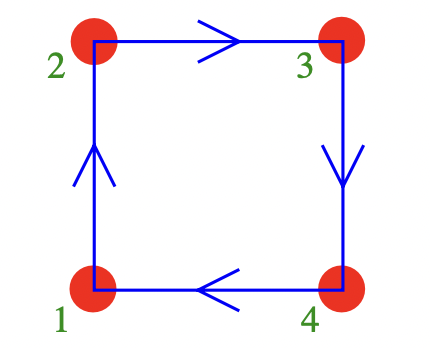
\includegraphics[scale=0.4]{Screen Shot 2022-07-13 at 11.21.15 AM.png}
	\caption{Plaquette: like "curl"}
	%\label{fig_nitjlogo2}
\end{figure}
Then the action will be,
\begin{align}
    S=&\sum_\Box \beta\left[1-\left(\frac{1}{n}\right)Re~Tr\left(U_{12}U_{23}U_{34}U_{41}\right)\right]\\
    =&\sum_\Box \beta\left[1-\left(\frac{1}{n}\right)Re~Tr\left(e^{\left(ig_0\int_{x_\mu_1}^{x_\mu_2}A_{\mu}.dx_{\mu}\right)}e^{\left(ig_0\int_{x_\mu_2}^{x_\mu_3}A_{\mu}.dx_{\mu}\right)}e^{\left(ig_0\int_{x_\mu_3}^{x_\mu_4}A_{\mu}.dx_{\mu}\right)}e^{\left(ig_0\int_{x_\mu_4}^{x_\mu_1}A_{\mu}.dx_{\mu}\right)}\right)\right]\\
    =&\sum_\Box \beta\left[1-\left(\frac{1}{n}\right)Re~Tr\left(exp{\left(ig_0\oint A_{\mu}.dx_{\mu}\right)}\right)\right]\\
    =&\sum_\Box \beta\left[1-\left(\frac{1}{n}\right)Re~Tr\left(exp{\left(ig_0\iint_s (\partial_\mu A_\nu-\partial_\nu A_\mu)ds\right)}\right)\right]\\
    =&\sum_\Box \beta\left[1-\left(\frac{1}{n}\right)Re~Tr\left(exp{\left(ig_0a^2 F_{\mu\nu}\right)}\right)\right]=\sum_\Box \beta\left[1-\left(\frac{1}{n}\right)Tr\left(\cos{\left(g_0a^2 F_{\mu\nu}\right)}\right)\right]\\
    =&\sum_\Box \beta\left[1-\left(\frac{1}{n}\right)\left(Tr(\mathbb{I}_{n\times n})-Tr\left(\frac{g^2_0a^4F^2_{\mu\nu}}{2}\right)+\mathcal{O}(a^8)\right)\right]\\
    =&\sum_\Box \frac{\beta g^2_0}{2n}Tr(F^2_{\mu\nu})a^4+\mathcal{O}(a^6)\\
    S=&\sum_\Box \frac{\beta g^2_0}{2n}\frac{1}{2}Tr(F_{\mu\nu}F_{\mu\nu})a^4+\mathcal{O}(a^6)
\end{align}

Then in the continuum limit $a\longrightarrow0$,
 \begin{align}
     S=& \frac{\beta g^2_0}{2n}\int\frac{1}{2}Tr(F_{\mu\nu}F_{\mu\nu})d^4x+\mathcal{O}(a^6)
 \end{align}
Thus we obtain the usual gauge theory action if we identify
\begin{align}
    \beta=\frac{2n}{g_0^2}
\end{align}

\section{THE MONTE CARLO METHOD} 
The lattice regularized quantum expectation value of an observable $\mathcal{O}(U_{ij})$ is given by
\begin{align}
    \braket{\mathcal{O}}&=Z^{-1}\int \prod_{ij}dU_{ij}\mathcal{O}(U_{ij})e^{-S(U_{ij},g)},\\
    Z&=\int \prod_{ij}dU_{ij}e^{-S(U_{ij},g)}
\end{align}
\begin{itemize}
    \item  An initial configuration $C^{(1)}$ is stored into the memory of the computer\footnote{Lattice Gauge Theories and Monte Carlo Simulations book by Claudio Rebbi }.        
    \item From $C^{(1)}$ the computer generates a new configuration $C^{(2)}$ which replaces $C^{(1)}$ in the memory, by a stochastic procedure.
    \item Transition probability $p(C\longrightarrow C')$ is defined for the passage between one configuration and the next. 
    \item From $C^{(2)}$ the computer generates a new configuration $C^{(3)}$, and so on, producing eventually a very large number of configurations. 
    \item Probability of encountering any definite configuration $C^(k)$ at larger $k$ steps converges to a distribution proportional to the correct measure factor $e^{-S(C)}$.
    \item Assuming that after $n_0$ steps the probability distribution has come close enough to the correct limiting one, we approximate the exact quantum expectation values by
    \begin{align}
        \braket{\mathcal{O}}=\frac{1}{n}\sum_{k=n_0+1}^{n}\mathcal{O}(C^{(k)})
    \end{align}
    \item The Boltzmann distribution $p(C) \propto e^{-S(C)}$ must be an eigenvector of the probability matrix $p(C \longrightarrow C')$. This is guaranteed if $p$ obeys detailed balance condition 
    \begin{align}
        \frac{p(C\longrightarrow C')}{p(C'\longrightarrow C)}=\frac{e^{-S(C')}}{e^{-S(C)}}
    \end{align}
    \item The transition matrix $p(C \longrightarrow C')$ is determined in two steps. First a new candidate configuration $C'$ is selected starting from $C$ according to some probability distribution $p_0(C\longrightarrow C')$, satisfying the equality 
    \begin{align}
        p_0(C\longrightarrow C')\Longrightarrow p_0(C'\longrightarrow C)
    \end{align}
    \item The variation in action $\vartriangle S=S(C')-S(C)$ that would be induced by the change is calculated. 
    \item A pseudo-random number is then selected with uniform probability distribution between 0 and 1 and: 
    \begin{itemize}
        \item if $r < e^{-\vartriangle S}$ the change is accepted — the new configuration in the sequence is C'.
        \item if $r > e^{-\vartriangle S}$ the change is rejected and the new configuration is again C.
    \end{itemize}
    \item In the Metropolis procedure, the transitions $P_0(C\longrightarrow C')$ and $P(C\longrightarrow C')$ can be further qualified, for a gauge system, as $P_0(U_{ji}\longrightarrow U_{ji}')$ and $P(U_{ji}\longrightarrow U_{ji}')$, all other $U_{ji}$ being kept fixed. 
\end{itemize}

\end{document}